% Options for packages loaded elsewhere
\PassOptionsToPackage{unicode}{hyperref}
\PassOptionsToPackage{hyphens}{url}
\PassOptionsToPackage{dvipsnames,svgnames,x11names}{xcolor}
%
\documentclass[
  12pt,
  letterpaper,
  DIV=11,
  numbers=noendperiod]{scrartcl}

\usepackage{amsmath,amssymb}
\usepackage{setspace}
\usepackage{iftex}
\ifPDFTeX
  \usepackage[T1]{fontenc}
  \usepackage[utf8]{inputenc}
  \usepackage{textcomp} % provide euro and other symbols
\else % if luatex or xetex
  \usepackage{unicode-math}
  \defaultfontfeatures{Scale=MatchLowercase}
  \defaultfontfeatures[\rmfamily]{Ligatures=TeX,Scale=1}
\fi
\usepackage{lmodern}
\ifPDFTeX\else  
    % xetex/luatex font selection
\fi
% Use upquote if available, for straight quotes in verbatim environments
\IfFileExists{upquote.sty}{\usepackage{upquote}}{}
\IfFileExists{microtype.sty}{% use microtype if available
  \usepackage[]{microtype}
  \UseMicrotypeSet[protrusion]{basicmath} % disable protrusion for tt fonts
}{}
\makeatletter
\@ifundefined{KOMAClassName}{% if non-KOMA class
  \IfFileExists{parskip.sty}{%
    \usepackage{parskip}
  }{% else
    \setlength{\parindent}{0pt}
    \setlength{\parskip}{6pt plus 2pt minus 1pt}}
}{% if KOMA class
  \KOMAoptions{parskip=half}}
\makeatother
\usepackage{xcolor}
\setlength{\emergencystretch}{3em} % prevent overfull lines
\setcounter{secnumdepth}{5}
% Make \paragraph and \subparagraph free-standing
\makeatletter
\ifx\paragraph\undefined\else
  \let\oldparagraph\paragraph
  \renewcommand{\paragraph}{
    \@ifstar
      \xxxParagraphStar
      \xxxParagraphNoStar
  }
  \newcommand{\xxxParagraphStar}[1]{\oldparagraph*{#1}\mbox{}}
  \newcommand{\xxxParagraphNoStar}[1]{\oldparagraph{#1}\mbox{}}
\fi
\ifx\subparagraph\undefined\else
  \let\oldsubparagraph\subparagraph
  \renewcommand{\subparagraph}{
    \@ifstar
      \xxxSubParagraphStar
      \xxxSubParagraphNoStar
  }
  \newcommand{\xxxSubParagraphStar}[1]{\oldsubparagraph*{#1}\mbox{}}
  \newcommand{\xxxSubParagraphNoStar}[1]{\oldsubparagraph{#1}\mbox{}}
\fi
\makeatother

\usepackage{color}
\usepackage{fancyvrb}
\newcommand{\VerbBar}{|}
\newcommand{\VERB}{\Verb[commandchars=\\\{\}]}
\DefineVerbatimEnvironment{Highlighting}{Verbatim}{commandchars=\\\{\}}
% Add ',fontsize=\small' for more characters per line
\usepackage{framed}
\definecolor{shadecolor}{RGB}{241,243,245}
\newenvironment{Shaded}{\begin{snugshade}}{\end{snugshade}}
\newcommand{\AlertTok}[1]{\textcolor[rgb]{0.68,0.00,0.00}{#1}}
\newcommand{\AnnotationTok}[1]{\textcolor[rgb]{0.37,0.37,0.37}{#1}}
\newcommand{\AttributeTok}[1]{\textcolor[rgb]{0.40,0.45,0.13}{#1}}
\newcommand{\BaseNTok}[1]{\textcolor[rgb]{0.68,0.00,0.00}{#1}}
\newcommand{\BuiltInTok}[1]{\textcolor[rgb]{0.00,0.23,0.31}{#1}}
\newcommand{\CharTok}[1]{\textcolor[rgb]{0.13,0.47,0.30}{#1}}
\newcommand{\CommentTok}[1]{\textcolor[rgb]{0.37,0.37,0.37}{#1}}
\newcommand{\CommentVarTok}[1]{\textcolor[rgb]{0.37,0.37,0.37}{\textit{#1}}}
\newcommand{\ConstantTok}[1]{\textcolor[rgb]{0.56,0.35,0.01}{#1}}
\newcommand{\ControlFlowTok}[1]{\textcolor[rgb]{0.00,0.23,0.31}{\textbf{#1}}}
\newcommand{\DataTypeTok}[1]{\textcolor[rgb]{0.68,0.00,0.00}{#1}}
\newcommand{\DecValTok}[1]{\textcolor[rgb]{0.68,0.00,0.00}{#1}}
\newcommand{\DocumentationTok}[1]{\textcolor[rgb]{0.37,0.37,0.37}{\textit{#1}}}
\newcommand{\ErrorTok}[1]{\textcolor[rgb]{0.68,0.00,0.00}{#1}}
\newcommand{\ExtensionTok}[1]{\textcolor[rgb]{0.00,0.23,0.31}{#1}}
\newcommand{\FloatTok}[1]{\textcolor[rgb]{0.68,0.00,0.00}{#1}}
\newcommand{\FunctionTok}[1]{\textcolor[rgb]{0.28,0.35,0.67}{#1}}
\newcommand{\ImportTok}[1]{\textcolor[rgb]{0.00,0.46,0.62}{#1}}
\newcommand{\InformationTok}[1]{\textcolor[rgb]{0.37,0.37,0.37}{#1}}
\newcommand{\KeywordTok}[1]{\textcolor[rgb]{0.00,0.23,0.31}{\textbf{#1}}}
\newcommand{\NormalTok}[1]{\textcolor[rgb]{0.00,0.23,0.31}{#1}}
\newcommand{\OperatorTok}[1]{\textcolor[rgb]{0.37,0.37,0.37}{#1}}
\newcommand{\OtherTok}[1]{\textcolor[rgb]{0.00,0.23,0.31}{#1}}
\newcommand{\PreprocessorTok}[1]{\textcolor[rgb]{0.68,0.00,0.00}{#1}}
\newcommand{\RegionMarkerTok}[1]{\textcolor[rgb]{0.00,0.23,0.31}{#1}}
\newcommand{\SpecialCharTok}[1]{\textcolor[rgb]{0.37,0.37,0.37}{#1}}
\newcommand{\SpecialStringTok}[1]{\textcolor[rgb]{0.13,0.47,0.30}{#1}}
\newcommand{\StringTok}[1]{\textcolor[rgb]{0.13,0.47,0.30}{#1}}
\newcommand{\VariableTok}[1]{\textcolor[rgb]{0.07,0.07,0.07}{#1}}
\newcommand{\VerbatimStringTok}[1]{\textcolor[rgb]{0.13,0.47,0.30}{#1}}
\newcommand{\WarningTok}[1]{\textcolor[rgb]{0.37,0.37,0.37}{\textit{#1}}}

\providecommand{\tightlist}{%
  \setlength{\itemsep}{0pt}\setlength{\parskip}{0pt}}\usepackage{longtable,booktabs,array}
\usepackage{calc} % for calculating minipage widths
% Correct order of tables after \paragraph or \subparagraph
\usepackage{etoolbox}
\makeatletter
\patchcmd\longtable{\par}{\if@noskipsec\mbox{}\fi\par}{}{}
\makeatother
% Allow footnotes in longtable head/foot
\IfFileExists{footnotehyper.sty}{\usepackage{footnotehyper}}{\usepackage{footnote}}
\makesavenoteenv{longtable}
\usepackage{graphicx}
\makeatletter
\newsavebox\pandoc@box
\newcommand*\pandocbounded[1]{% scales image to fit in text height/width
  \sbox\pandoc@box{#1}%
  \Gscale@div\@tempa{\textheight}{\dimexpr\ht\pandoc@box+\dp\pandoc@box\relax}%
  \Gscale@div\@tempb{\linewidth}{\wd\pandoc@box}%
  \ifdim\@tempb\p@<\@tempa\p@\let\@tempa\@tempb\fi% select the smaller of both
  \ifdim\@tempa\p@<\p@\scalebox{\@tempa}{\usebox\pandoc@box}%
  \else\usebox{\pandoc@box}%
  \fi%
}
% Set default figure placement to htbp
\def\fps@figure{htbp}
\makeatother

\RequirePackage{natbib}
% Add all necessary packages here
\usepackage{amsmath,amssymb,epsfig,tabularx,wrapfig}
\usepackage{graphicx}
\usepackage{color,soul}
\usepackage{verbatim}
\usepackage{ifthen}
\usepackage{psfrag}
\usepackage{siunitx}
\usepackage{enumerate}
\usepackage{hyperref}
\usepackage{setspace}
\usepackage{natbib}
% Formatting
\setlength{\topmargin}{-.5 in}
\setlength{\textheight}{9. in}
\setlength{\oddsidemargin}{.1in}
\setlength{\evensidemargin}{-.35in}
\setlength{\textwidth}{6in}
\font\heada=cmbx10 scaled\magstep3
\font\headb=cmsl10 scaled\magstep1
\font\headc=cmr8
\pretolerance=10000
\raggedright
\setlength{\parindent}{2 em}

% Define new commands
\newcommand{\bm}{\mathbf}
\newcommand{\PR}{\mathrm{P}}
\newcommand{\R}{\mathbb{R}}

\newcommand{\todo}[1]{\payAttention{red}{TODO}{#1}}

% Identifying information
\newcommand{\myname}{Ben DeVries}
\newcommand{\myadvisor}{Andy Hoegh}
\newcommand{\wprojcoord}{Ian Laga}  % Current Writing Project Coordinator
\newcommand{\maintitle}{YOUR TITLE HERE}
\newcommand{\mydate}{Date of completion here as Month Day, Year}

\KOMAoption{captions}{tableheading}
\makeatletter
\@ifpackageloaded{caption}{}{\usepackage{caption}}
\AtBeginDocument{%
\ifdefined\contentsname
  \renewcommand*\contentsname{Table of contents}
\else
  \newcommand\contentsname{Table of contents}
\fi
\ifdefined\listfigurename
  \renewcommand*\listfigurename{List of Figures}
\else
  \newcommand\listfigurename{List of Figures}
\fi
\ifdefined\listtablename
  \renewcommand*\listtablename{List of Tables}
\else
  \newcommand\listtablename{List of Tables}
\fi
\ifdefined\figurename
  \renewcommand*\figurename{Figure}
\else
  \newcommand\figurename{Figure}
\fi
\ifdefined\tablename
  \renewcommand*\tablename{Table}
\else
  \newcommand\tablename{Table}
\fi
}
\@ifpackageloaded{float}{}{\usepackage{float}}
\floatstyle{ruled}
\@ifundefined{c@chapter}{\newfloat{codelisting}{h}{lop}}{\newfloat{codelisting}{h}{lop}[chapter]}
\floatname{codelisting}{Listing}
\newcommand*\listoflistings{\listof{codelisting}{List of Listings}}
\makeatother
\makeatletter
\makeatother
\makeatletter
\@ifpackageloaded{caption}{}{\usepackage{caption}}
\@ifpackageloaded{subcaption}{}{\usepackage{subcaption}}
\makeatother

\usepackage[]{natbib}
\bibliographystyle{plainnat}
\usepackage{bookmark}

\IfFileExists{xurl.sty}{\usepackage{xurl}}{} % add URL line breaks if available
\urlstyle{same} % disable monospaced font for URLs
\hypersetup{
  pdftitle={DeVries Writing Project},
  colorlinks=true,
  linkcolor={blue},
  filecolor={Maroon},
  citecolor={Blue},
  urlcolor={Blue},
  pdfcreator={LaTeX via pandoc}}


\title{DeVries Writing Project}
\author{}
\date{}

\begin{document}
\maketitle

%%%%%%%%%%%%%%%%%%%%%%%%%%%%%%%%%%%%%%%%%%%%
% Title page
\begin{singlespace}

\begin{titlepage}
\null
\vspace{2.in}
% Enter title here
\begin{center}
{\LARGE\bfseries \maintitle} \vspace{.1in}

\vspace{.05in}
{\LARGE\bfseries $\;$} \\ [.5in]
{\Large  \myname \\
\vspace{0.5cm}
Department of Mathematical Sciences \\
Montana State University \\ [.5in]}
\mydate \\ [1.in]
A writing project submitted in partial fulfillment\\
of the requirements for the degree\\[.25in]
Master of Science in Statistics
\end{center}
\end{titlepage}

%%%%%%%%%%%%%%%%%%%%%%%%%%%%%%%%%%%%%%%%%%%%
% Signatures
\begin{titlepage}
\null
\vspace{2.in}
\begin{center}
{\bfseries\huge APPROVAL}\\[1.in]
of a writing project submitted by\\[.25in]
\myname \\[1.in]
\end{center}
\noindent
This writing project has been read by the writing project advisor and
has been found to be satisfactory regarding content, English usage,
format, citations, bibliographic style, and consistency, and is ready
for submission to the Statistics Faculty.

\vspace{.3in}
\begin{center}
\begin{tabular}{ll}
\rule{2.75in}{.03in} & \rule{2.75in}{.03in} \\
Date& \myadvisor \\
& Writing Project Advisor \\
\end{tabular}
\end{center}

\vspace{1cm}

\begin{center}
\begin{tabular}{ll}
\rule{2.75in}{.03in} & \rule{2.75in}{.03in} \\
Date& \wprojcoord \\
& Writing Projects Coordinator \\
\end{tabular}
\end{center}

\end{titlepage}
\end{singlespace}


%%%%%%%%%%%%%%%%%%%%%%%%%%%%%%%%%%%%%%%%%%%%
% Abstract
\vspace{2.in}
\begin{abstract}
\begin{doublespace}
This is my abstract. Note that I'm using line breaks without trailing white spaces in this .tex file to
make version control work better. The XXXX is an important problem for researchers and this writing
project was written to provide a solution to this important problem. It contains an exploration
of the history of the problem, motivating its importance, an exploration of an application to
illustrate its importance, development and/or discussion of statistical software to apply
the solutions to the problem, a simulation study to explore the performance of the methods,
and a conclusion. It also contains useful references and an appendix containing code used.
Or maybe it doesn't do all this - it depends on what you do for your project.
\end{doublespace}
\end{abstract}


\newpage


\renewcommand*\contentsname{Table of contents}
{
\hypersetup{linkcolor=}
\setcounter{tocdepth}{3}
\tableofcontents
}

\setstretch{2}
\newpage

\section{Introduction}\label{sec:intro}

Statistical Modelling: the Two Cultures \citep{Breiman_2001} describes
two approaches to data problems; data, and algorithmic models. Data
modelling is described as classical statistics where data is assumed to
be generated by some stochastic process. For some problems, the true
underlying process contains complex dynamics that may or may not be
observable. In algorithmic modelling, we don't try to find the true
model. Instead, the goal is to find a generalizable approximation. For
this project we focus on applications of tree based models.

\subsection{Subsection}\label{subsection}

This is a subsection in my Introduction section.

\section{Background}\label{sec:background}

\subsection{Supervised Learning}\label{supervised-learning}

With this project, we chose to focus on tree based methods. The Elements
of Statistical Learning \citep{esl} was a key source for understanding
algorithms and concepts in statistical learning. Our backgroun
discussion begins with some notation and concepts in supervised
learning. We then discuss the algorithms for several models, using
simulation to demonstrate there use. In supervised learning problems we
work to map a set of features to a target. When discussing these
components, we'll follow the notation used in The Elements of
Statistical Learning \citep{esl}. \(X\) denotes the features while \(Y\)
and \(G\) denote the target for quantitative and categroical responses
respectively. If there are \(N\) observations of \(p\) inputs, then
\(\bm X\) is an \(N\times p\) matrix. The inputs for the \(i\)'th
observation are \(\bm x_i\) while \(\bm x_j\) denotes the vector of all
observations for the \(j\)'th input. A common approach in supervised
learning is to assume our featurs and target are observation of random
variables with joint distribution \(\text{Pr}(Y,X)\). \(G\) would
replace \(Y\) in a classification problem and \(\bm X\) would replace
\(X\) for multiple covariates. We want to find a function
\(f:\mathcal{X}\rightarrow\mathcal{Y}\) that predicts \(Y\) reasonably
well. To do this, we define a loss function \(L(Y,f(X))\) which
penalizes the prediction error on a training set
\(\bm \tau=(x_i,y_i),\ i=1,2,...,N\). The expected prediction error
(EPE) is defined as \(\mathbb{E}[L(Y,f(X))]\). Our overall goal is to
approximate the function \(f\) that minimizes the EPE. Using squared
errors for loss \((L_2)\), the EPE is minimized by choosing \(f\) such
that \(f(x)=\mathbb{E}[Y|X=x]\) (The Elments of Statistical Learning,
pg. 18 \citep{esl}). Now we need an algorithm to approximate \(f\) using
\(\bm \tau\). Choosing an appropriate algorithm will be heavily
influenced by the availability and distribution of data. With a
quantitative target, we might be able to assume an additive error
relationship between \(Y\) and \(\bm X\). The additive error model is
simply \(Y=f(\bm X)+\epsilon\) where \(\mathbb{E}[\epsilon]=0\) and
\(\bm X\perp\epsilon\). Here we are assuming the process that generated
\(Y\) can be approximated using \(\bm X\) such that the error due to
ignored features and other factors has mean zero. For data that was
generated under an additive error model, a natural approach to
approximate \(f\) is to use a sum of basis functions. The additive model
is defined as \(Y=\beta_0+\sum_{j=1}^pf_j(\bm x_j)+\epsilon\). In this
model, each \(f_j\) could be a sum of basis functions. The major
limitation to an additive model is we assume no interactions between
features. There's no reason we can't add interactions or functions of
multiple covariates, but identifying these interactions is difficult. We
might be able to fit a model with select select transformations of
covariates and every possible interaction, but this would almost
certainly result in overfitting. Assuming a generating model with any
form of noise implies even the optimal \(f\) will not predict every
observation perfectly. A model is overfit when global trends are ignored
to explain slight irregularities in a sample. Discerning irregularities
is highly subjective. Any decision we make based on observed data may
lead to overfitting. Remember our overall goal is to minimize the EPE
but unfortunately the EPE is not quantifiable as we do not know the true
distribution of \(Y|X\). Like any other problem in statistics concerning
an unknown quantity, the solution is to use estimates based on a sample.
To obtain our estimate, we use some form of cross validation. There are
a variety of methods to perform cross validation, but the two most
common are hold out and K-fold. In hold out, some portion of the data is
held out for testing and the rest is used to fit the model. If the model
contains hyper parameters, we could split the data into training,
validation, and testing. Fitting models to the training set, we can try
various values for hyper parameters and compare model performance for
predictions on the validation set. After we determine the optimal hyper
parameter values, we refit the model on the combined training and
validation set before using the testing set to assess the final fit.
Using training/testing splits is generally favored for computationally
intensive problems with many observations. The hold out method gives us
a single sample to estimate the prediction error. In K-fold cross
validation we partition the observations into \(K\) folds, resulting in
\(K\) samples of size \(n/K\). A model is fit using all but one fold
which is held for testing. The process is then repeated until all folds
and thus all observations have been tested. More observations generally
implies a better estimate, but refitting models may change estimates.
K-fold does not estimate the prediction error of the final estimated
model, but still provides some idea of how the model will perform on new
data. K-fold is an excellent tool for tuning models prior to testing. So
far we have discussed a general approach to problems centered around
prediction. In the next subsection we explore the intuition behind two
algorithms to approximate \(f\), decision trees and random forests.
Later, we turn our attention to tree based models fit with Bayesian
methods. Our discussion of Bayesian tree models is primarily centered
around Bayesian Additive Regression Trees (BART), but a discussion of
predecessors is included.

\subsection{Decision Trees}\label{decision-trees}

Decision trees are a type of hierarchical model where the the feature
space is partitioned into hyperrectangular regions, and a model is fit
for each region. For regression tasks, we typically use mean only
models. In this case the decision tree model is a step function. Unlike
our mean only models for linear regression, we do not make any
distributional assumptions. Without a distribution, we can't quantify
the uncertainty in our predictions or the decision boundaries.
Additionally, the binary structure of trees makes the effects of
individual predictors less interpretable than a linear model. Small
changes in a feature \(x_{i,j}\) may not effect the associated
prediction \(\hat y_i\). On the other hand, trees greatly outperform
linear models with more complex data. The hierarchical structure
naturally handles multicollinearity, and can help us find interactions
between covariates. Even though we don't believe \(\bm X\) is related to
\(\bm y\) by a step function, we can gain insight to the true
relationship by a step function approximation. An example of a tree
model is shown in Figure~\ref{fig-tree-examp}. Every decision after the
top root node is conditioned on the previous decisions, allowing us to
display the hierarchy graphically.

\begin{figure}

\centering{

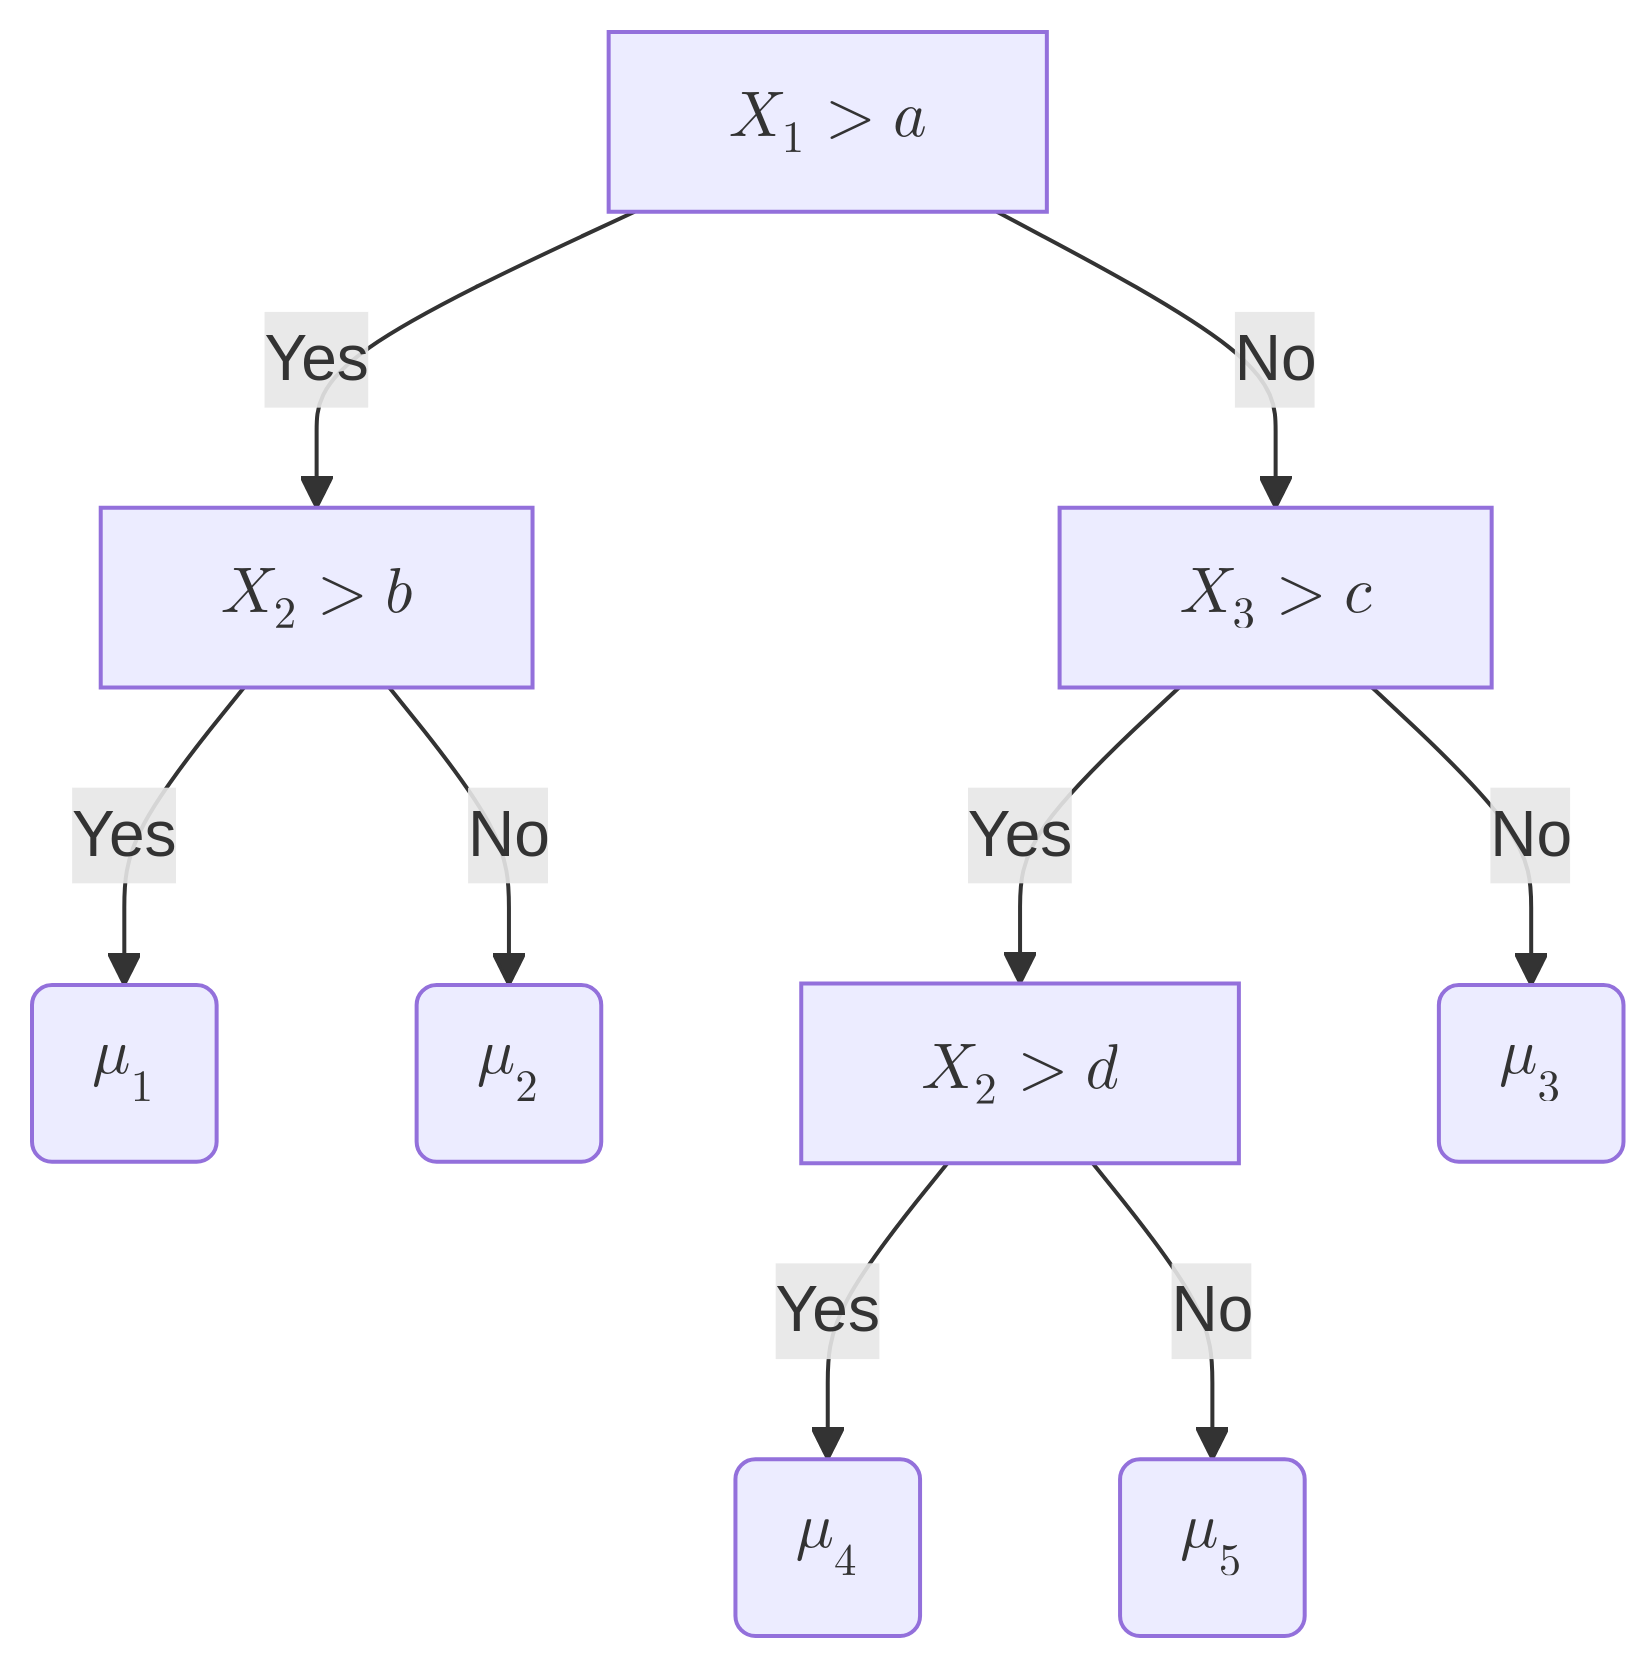
\includegraphics[width=4.31in,height=4.34in]{main_QMD_files/figure-latex/mermaid-figure-1.png}

}

\caption{\label{fig-tree-examp}Visualization of binary decision tree}

\end{figure}%

Step functions are very flexible and for any training set \(\bm X\) with
target \(Y\) where \(y_i|\bm X_i= y_j|\bm X_i\) for all \(i,j\), we can
fit a tree that will have no error on the training set. With this
flexibility, over fitting is a major concern. We can control the overall
size and shape of trees with three hyper-parameters. First is the
complexity parameter \(\alpha\). \(\alpha\) scales the penalty which is
based on the number of terminal nodes (mean only models). Next we have
the minimum split and minimum bucket sizes. The minimum bucket is the
fewest number of observations allowed in a terminal node. Similarly, the
minimum split is the least number of observations allowed in one outcome
of a binary decision. We generally choose the complexity parameter by
growing the largest possible tree, then removing terminal nodes with
fewer observations. Next we compare the trees via cross validation and
choose the tree with minimal cross validated error. This process of
choosing an appropriate tree size is commonly referred to as pruning.
While pruning helps reduce the risk of over fitting, large regression
trees are inherently unstable. We'll demonstrate this with data
simulated under the model described below. A simulated testing data set
displaying the true function along with the fit from a tree chosen by
cross validation on training is displayed in
Figure~\ref{fig-sim1-pred-vis}. Figure~\ref{fig-sim1-tree} displays the
number of splits for the optimal complexity parameter chosen by cross
validation.
\[y_i=\cos(108t_i\sin(108t_i+w_i))\cdot\exp(\sin(108t_i\cos(108t_i+x_i)))+z_i\]
\[W_i,X_i,Z_i\sim N(0,\sigma^2)\]
\[t_i=-\frac{\pi}{18},...,\frac{\pi}{18}\] \[i=1,2,...,350\]

\begin{figure}

\centering{

\pandocbounded{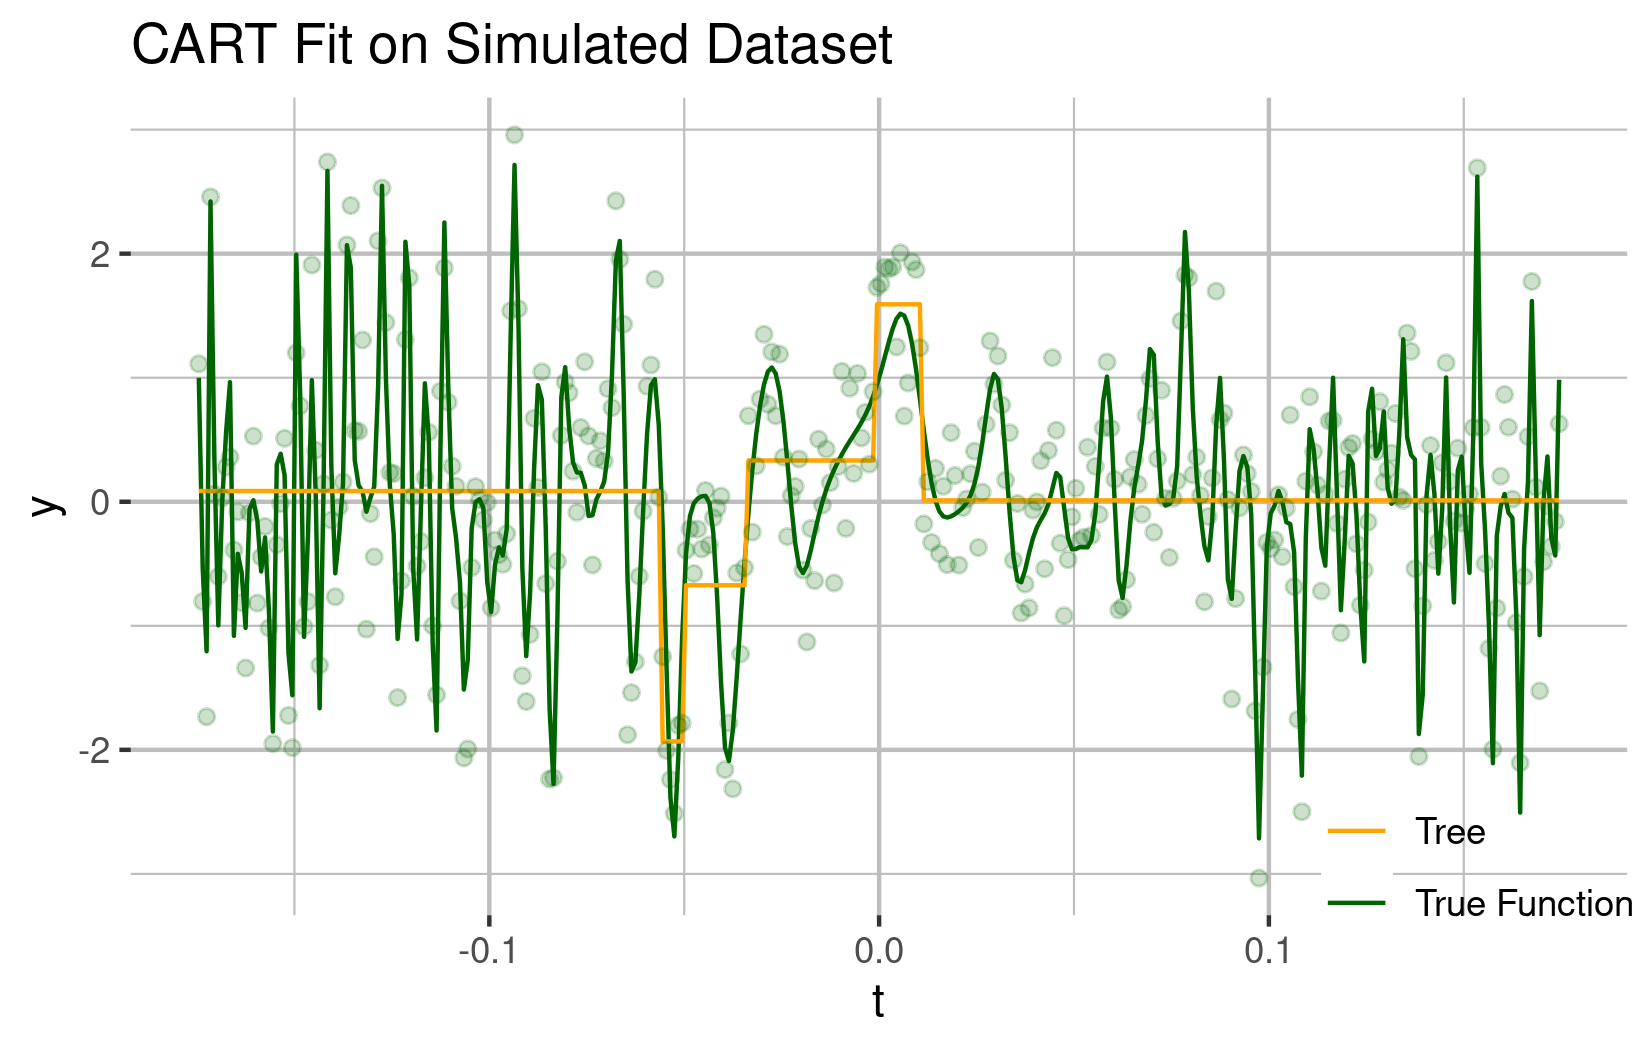
\includegraphics[keepaspectratio]{main_QMD_files/figure-pdf/fig-sim1-pred-vis-1.png}}

}

\caption{\label{fig-sim1-pred-vis}Visualization of simulated data and
predictions}

\end{figure}%

\begin{figure}

\centering{

\pandocbounded{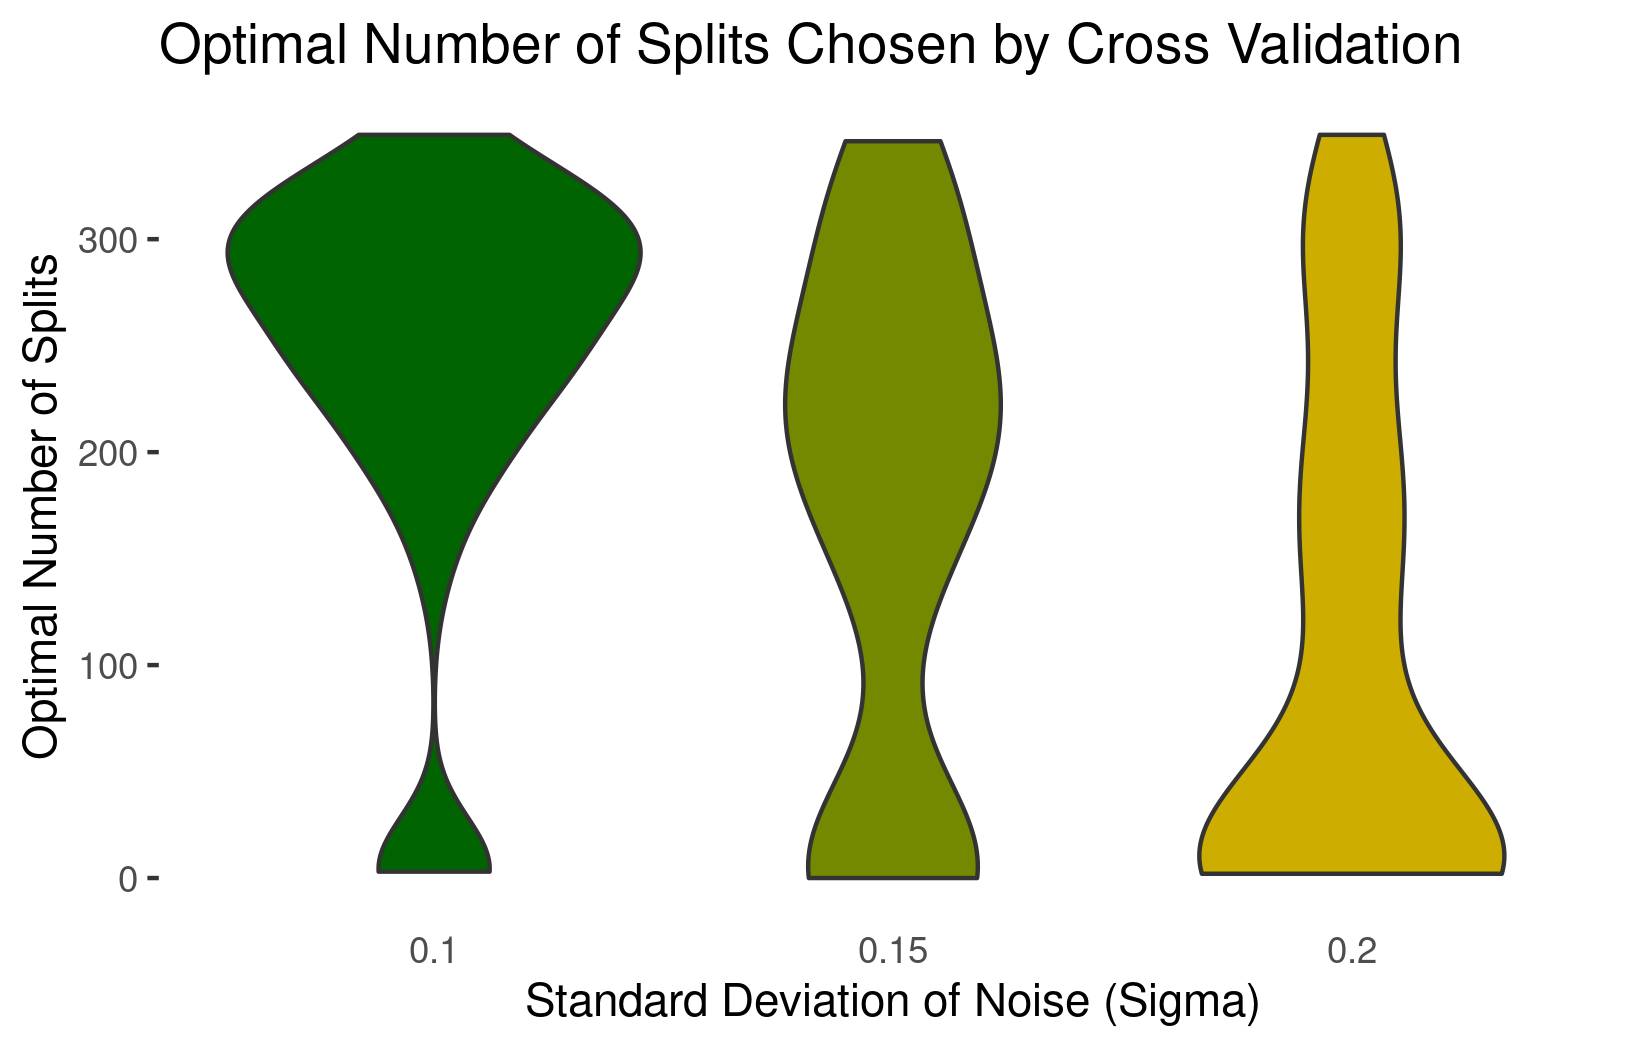
\includegraphics[keepaspectratio]{main_QMD_files/figure-pdf/fig-sim1-tree-1.png}}

}

\caption{\label{fig-sim1-tree}Violin plots of optimal number of splits
for simulated data}

\end{figure}%

Decision trees are very unstable for this data. Across all three noise
levels, the number of splits chosen by cross validation ranges from zero
to over 300. The variability in the size/structure of trees suggest we
can't have much faith in predictions from an individual tree. This led
to the development of the random forest algorithm by Leo Breiman and
Adele Cutler. Random forests are an adaptation of bagging. Bagging is
simply averaging the predictions of models fit to bootstrapped samples.
This reduces the variability of predictions at the cost of bias. The
random forest algorithm randomly selects subsets of all the available
predictors and fits decision tree to bootstrapped samples. A fitted
value \(y_i|\bm x_i\) is obtained by averaging predictions from all
trees where \(\bm x_i\) was not in the bootstrap sample. Combining many
trees, our estimated model is still a step function, but appears much
smoother than trees. This leads to more stable predictions as seen in
Figure~\ref{fig-sim1-mse}.

\begin{figure}

\centering{

\pandocbounded{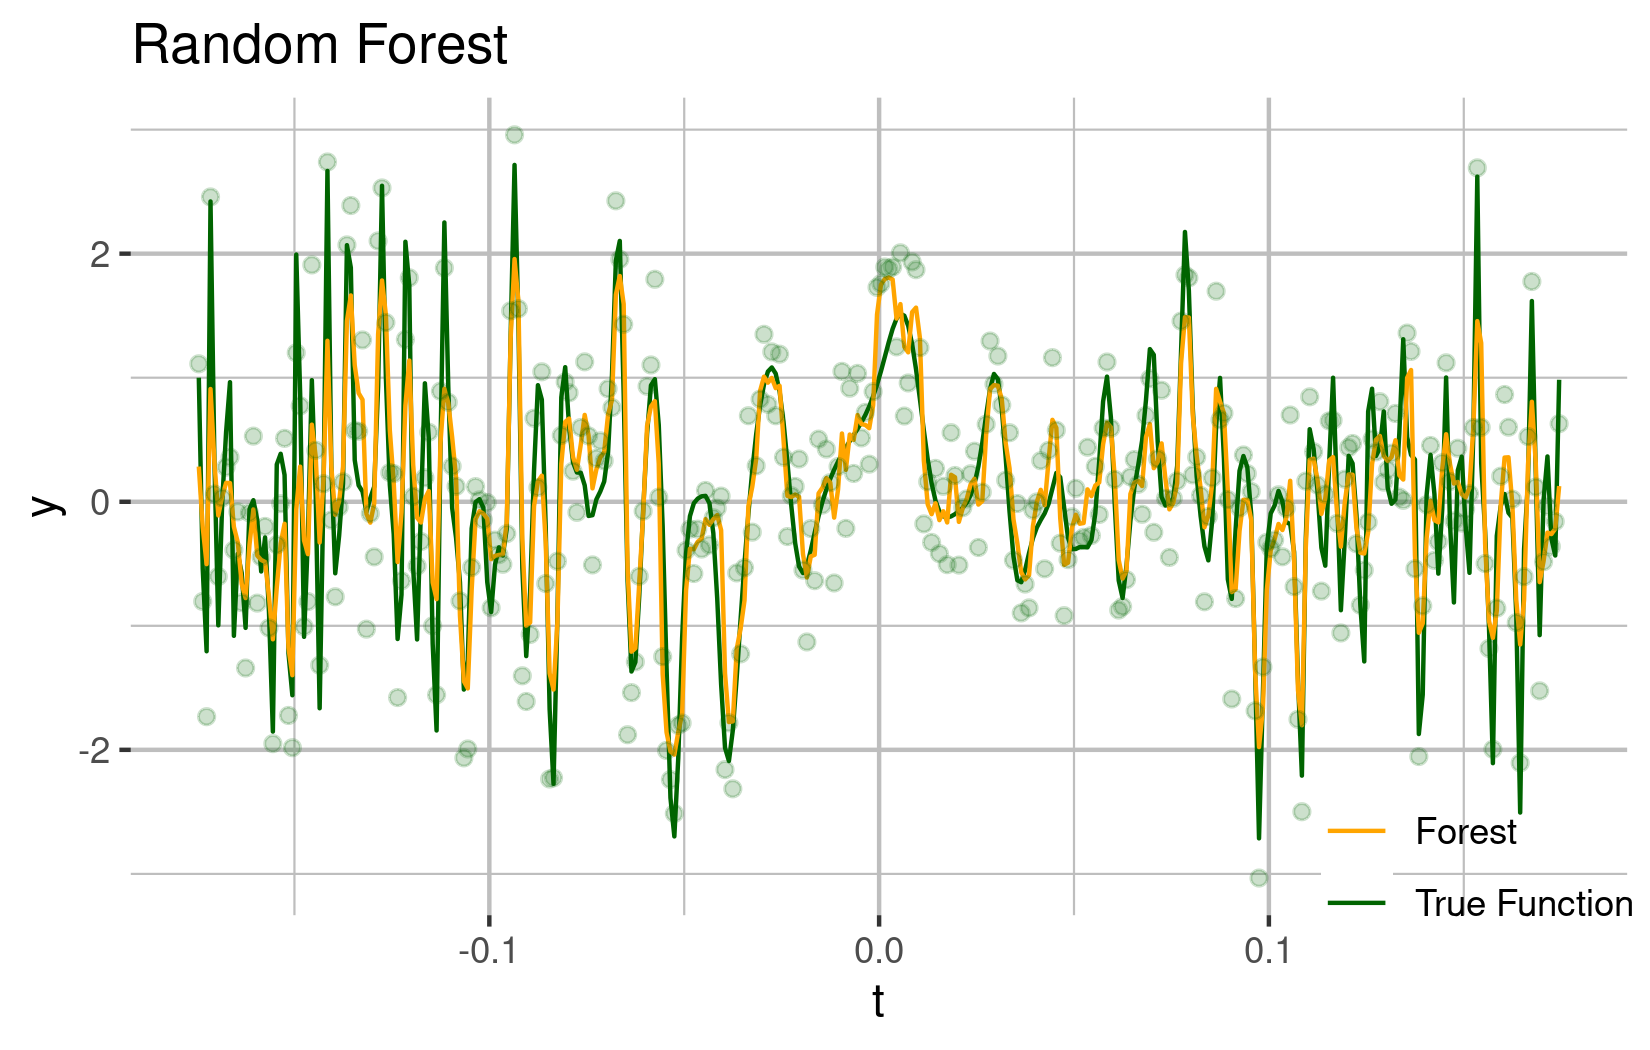
\includegraphics[keepaspectratio]{main_QMD_files/figure-pdf/fig-sim1-rf-fit-1.png}}

}

\caption{\label{fig-sim1-rf-fit}Violin plots of MSE for tree and forest
models on simulated data}

\end{figure}%

\begin{figure}

\centering{

\pandocbounded{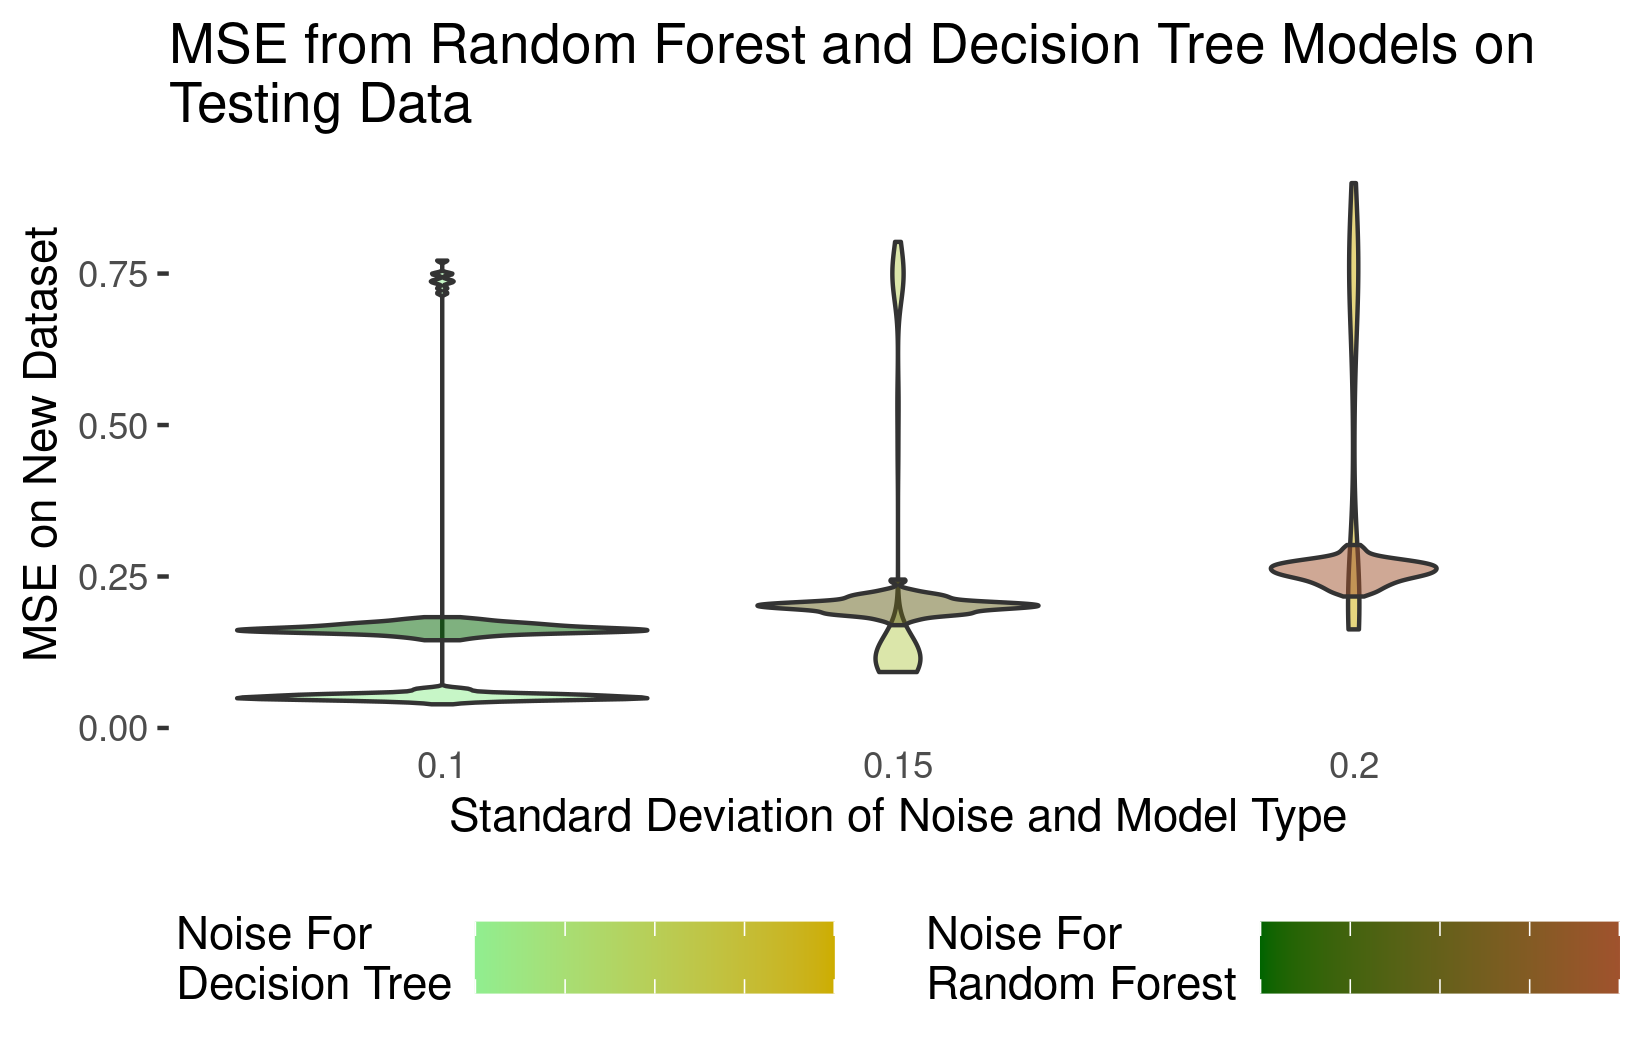
\includegraphics[keepaspectratio]{main_QMD_files/figure-pdf/fig-sim1-mse-1.png}}

}

\caption{\label{fig-sim1-mse}Violin plots of MSE for tree and forest
models on simulated data}

\end{figure}%

We see considerably less variation in the mean squared error of random
forests fit to the same data as individual decision trees, but single
tree models generally outperformed a random forest. Random forests are
designed for data with several covariates. With a single predictor, the
random forest algorithm degenerates to bagging with out of bag
predictions. Bagging reduces the variance of predictions at the cost of
bias, and thus the ``random forest'' predictions were often worse than
predictions from individual trees. Pages 600, 601 of \citep{esl} display
a proof showing that the bias of a random forest is the same as the bias
of any individual tree in the ensemble. The randomization in the random
forest algorithm implies trees within the ensemble are almost certainly
smaller than a single tree fit to the data. In cases where we have
access to several predictors, large trees will create complex
hierarchies that are unlikely to exist in the true model. The following
simulation study shows the random forest algorithm consistently
outperform a single tree for data generated under a linear model with
correlated covariates. Violin plots of MSE on testing data are displayed
in Figure~\ref{fig-sim2}.

\begin{figure}

\centering{

\pandocbounded{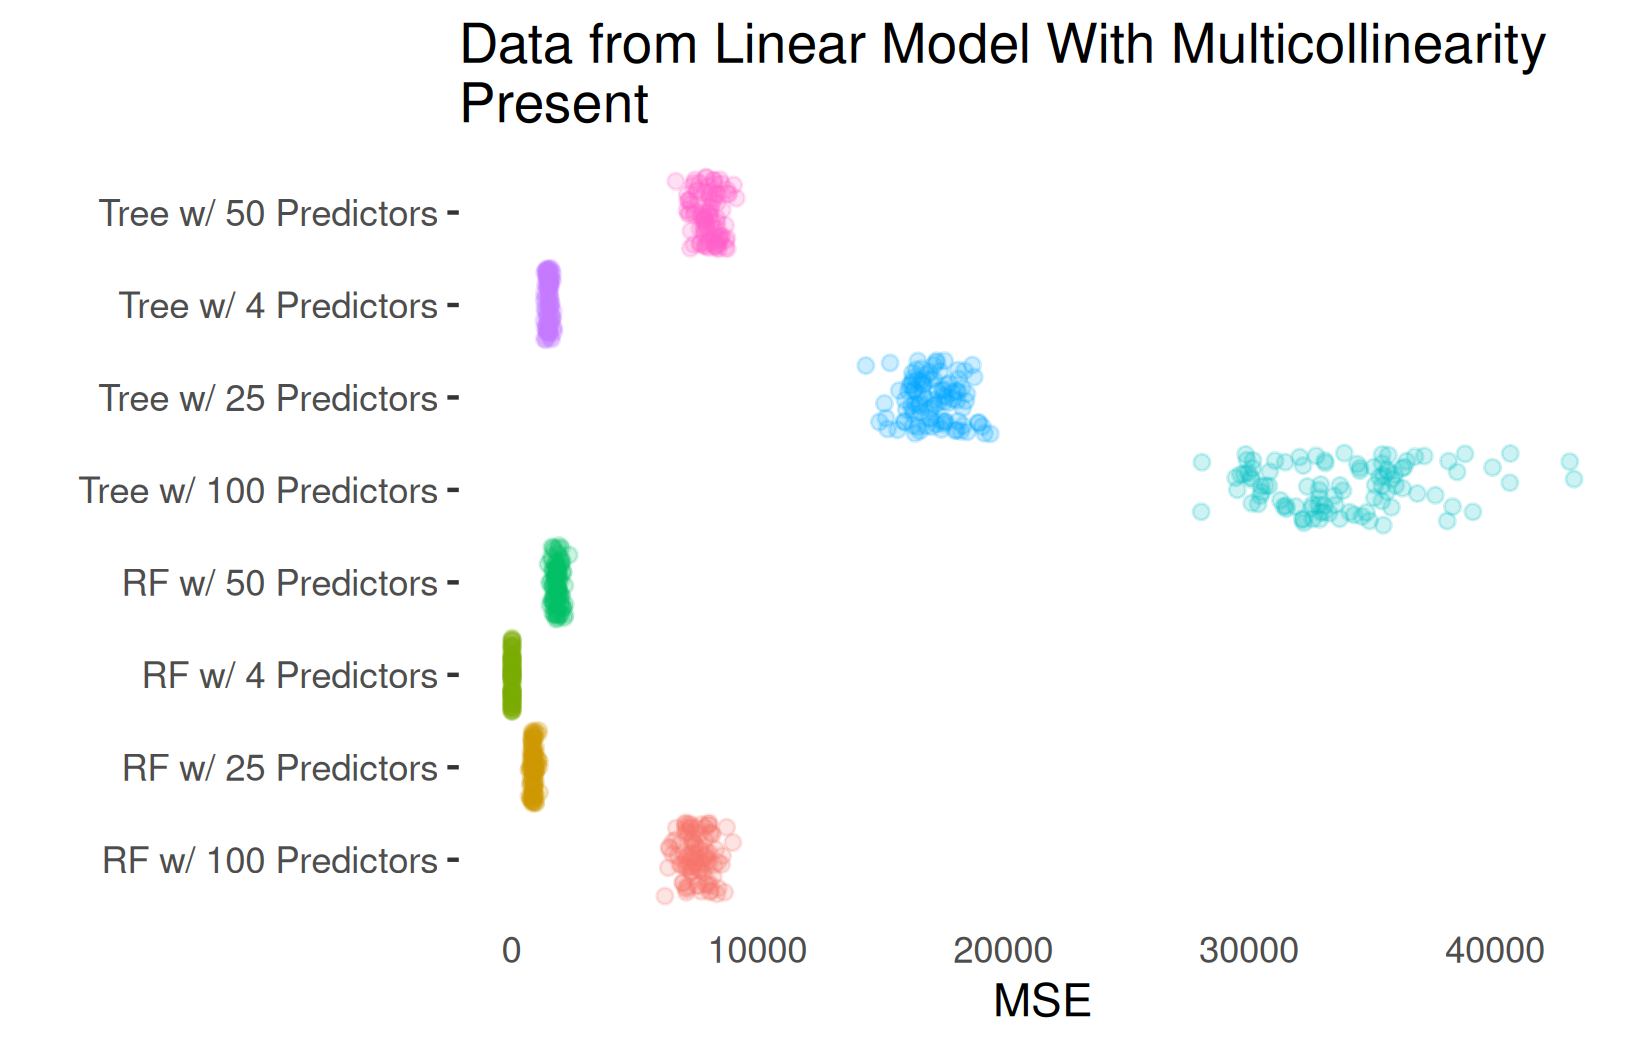
\includegraphics[keepaspectratio]{main_QMD_files/figure-pdf/fig-sim2-1.png}}

}

\caption{\label{fig-sim2}Violin plots of MSE for tree and forest models
on linear model with several predictors}

\end{figure}%

\subsection{Bayesian Trees}\label{bayesian-trees}

In the current and following section we discuss Bayesian methods for
tree algorithms, beginning with Bayesian Classification And Regression
Trees. Here, we briefly discuss the Bayesian approach to a regression
tree. There are many ways to specify a Bayesian tree, but we'll focus on
models developed by doctors Hugh Chipman, Edward George, and Robert
Mcculoch. Chipman et al.s \#\# Bayesian Additive Regression Trees (BART)
The other learning algorithm we explored was BART, or Bayesian Additive
Regression Trees. Introduced by Chipman et al \citep{bart_paper}, BART
is a flexible nonparametric regression method that combines the
strengths of decision trees and Bayesian modeling. For a continuous
predictor, BART assumes
\(y_i\sim N(\sum_{b=1}^m g(\bm x_i;T_b,M_b), \sigma^2)\) where \(T_b\)
is the \(b\)'th tree, \(M_b\) are the associated terminal nodes, and
\(g(\bm x_i;T_b,M_b)\) is the function that assigns \(\bm x_i\) to
\(\mu_{lb}\), \(l\in\{1,2,...,|M_b|\}\). Unlike the random forest
algorithm, the trees are not bagged and each tree has access to each
feature. The algorithm starts by growing \(M\) trees with a single
terminal node (stumps). Gibbs sampling is used to iteratively update
each tree conditioned on all other trees. Highly informative priors
prevent any single tree from dominating the model. BART assumes
independent priors for the trees and standard deviation. The joint prior
is given by
\[p((T_1, M_1), (T_2, M_2),...,(T_m, M_m),\sigma^2)=p(\sigma^2)\prod_{b=1}^mp(M_b|T_b)p(T_b)\]
where \(p(M_b|T_b)=\prod_{l=1}^{|M_b|}p(\mu_{lb}|T_b)\), and
\(p(\sigma^2)\sim\nu\lambda/\chi^2_\nu\) with hyperparameters
\(\nu,\lambda\). The hyper parameters are selected by first choosing a
point estimate \(\hat\sigma\). By default, this is the residual standard
deviation for a multiple linear regression model. \(\nu\) is then fixed
(\(\nu\in[3,10]\) reccomended) and \(\lambda\) solved for by imposing
the constraint \(\text{Pr}(\sigma<\hat\sigma)=q\), where \(q\) is an
additional hyper parameter. In the prior for a tree \(p(T_b)\), the
probability that a node at depth \(d\in\mathbb{N}\) is non-terminal is
given by \(\alpha(1+d)^{-\beta}\),
\(\alpha\in(0,1),\ \beta\in[0,\infty)\). A discrete uniform prior
imposes the initial belief that each feature equally likely to be
selected for a nodes splitting rule. Similarly, a discrete uniform
across the observed values of the selected predictor serves as the prior
for the cut point in the binary decision. A
\(N(|M|\mu_\mu,|M|\sigma^2_\mu)\) prior is assumed for each
\(\mu_{lb}|T_b\) where \(|M|\) is the total number of terminal nodes
across all trees. The hyperparameters \(\mu_\mu\) and \(\sigma_\mu\) are
chosen based on the data such that
\(\min(Y)=|M|\mu_\mu-k\sqrt{|M|}\sigma_mu\) and
\(\max(Y)=|M|\mu_\mu-k\sqrt{|M|}\sigma_\mu\). In \citep{bart_paper},
they reccomend choosing \(k\in[1,3]\). The BART R package rescales \(Y\)
such that \(Y\in[-0.5, 0.5]\) and chooses
\(\mu_\mu=0\implies\sigma_\mu=\frac{0.5}{k\sqrt{|M|}}\). One downside to
this is we are no longer utilizing out of bag predictions so we need a
testing set to quantify model performance. We also note that BART is not
a fully bayesian model as the number of trees \(m\) is fixed and data is
used to inform priors. Even if the model isn't fully Bayesian, we can
leverage the MCMC samples to obtain a posterior predictive distribution.
Hyper parameters can then be tuned using a testing set with the goal of
bringing prediction intervals to the nominal level. Another major
advantage to BART is the trees are smaller than in random forests due to
the regularizing prior. While BART is still a black box, we may be able
to draw potential associations between the features and target. Small
trees are easy to interpret and the posterior distribution of \(\mu\)'s
provides probabilities from which we can infer the importance of
features. An example of BART fit to the same simulated data used in
Figure~\ref{fig-sim1-pred-vis} is displayed in
Figure~\ref{fig-bart-sim1}. Choosing
\(m=250,k=0.6,\alpha=0.99,\beta=0.5,\hat\sigma=2\sqrt{\mathbb{V}[Y]}\)
resulted in a 95\% prediction interval within 1\% of nominal coverage on
the testing data for which parameters were tuned.

\begin{verbatim}
[1] 0.3415504
\end{verbatim}

\begin{verbatim}
[1] 0.3848066
\end{verbatim}

\begin{figure}

\centering{

\pandocbounded{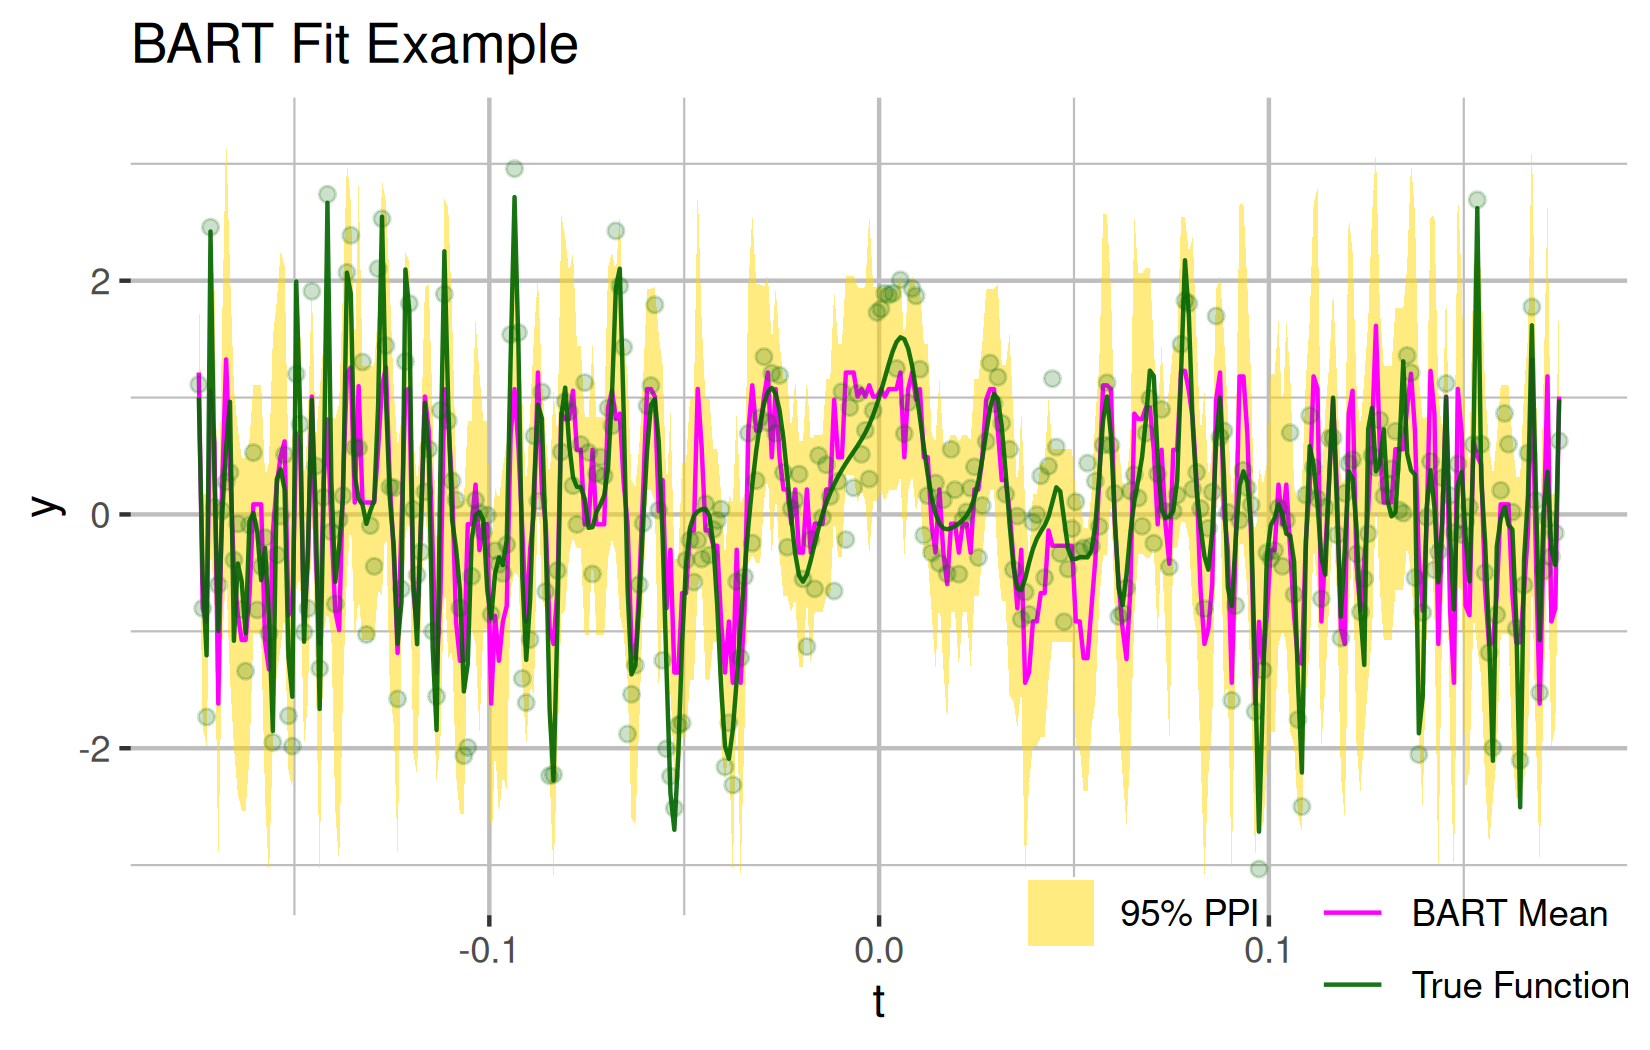
\includegraphics[keepaspectratio]{main_QMD_files/figure-pdf/fig-bart-sim1-1.png}}

}

\caption{\label{fig-bart-sim1}Visualization of bart}

\end{figure}%

\begin{Shaded}
\begin{Highlighting}[]
\NormalTok{modis }\OtherTok{\textless{}{-}} \FunctionTok{raster}\NormalTok{(}\StringTok{"\textasciitilde{}/Downloads/modis\_landcover2023.tif"}\NormalTok{)}
\NormalTok{modis\_df }\OtherTok{\textless{}{-}} \FunctionTok{as.data.frame}\NormalTok{(modis, }\AttributeTok{xy =}\NormalTok{ T) }\SpecialCharTok{|\textgreater{}} 
  \FunctionTok{mutate}\NormalTok{(}\AttributeTok{land\_cover =} \FunctionTok{factor}\NormalTok{(LC\_Type2, }\AttributeTok{labels =} \FunctionTok{c}\NormalTok{(}
    \StringTok{"Water Bodies"}\NormalTok{, }\StringTok{"Evergreen Needleleaf Forests"}\NormalTok{, }\StringTok{"Evergreen Broadleaf Forests"}\NormalTok{,}
    \StringTok{"Mixed Forests"}\NormalTok{, }\StringTok{"Open Shrublands"}\NormalTok{, }\StringTok{"Woody Savannas"}\NormalTok{, }\StringTok{"Savannas"}\NormalTok{, }\StringTok{"Grasslands"}\NormalTok{,}
    \StringTok{"Croplands"}\NormalTok{, }\StringTok{"Urban and Built{-}up Lands"}

\NormalTok{  )))}
\NormalTok{modis\_pal }\OtherTok{\textless{}{-}} \FunctionTok{c}\NormalTok{(}
  \StringTok{"Water Bodies"} \OtherTok{=} \StringTok{"\#1c0dff"}\NormalTok{,}
  \StringTok{"Evergreen Needleleaf Forests"} \OtherTok{=} \StringTok{"\#05450a"}\NormalTok{,}
  \StringTok{"Evergreen Broadleaf Forests"} \OtherTok{=} \StringTok{"\#086a10"}\NormalTok{,}
  \StringTok{"Deciduous Broadleaf Forests"} \OtherTok{=} \StringTok{"\#78d203"}\NormalTok{,}
  \StringTok{"Mixed Forests"} \OtherTok{=} \StringTok{"\#009900"}\NormalTok{,}
  \StringTok{"Closed Shrublands"} \OtherTok{=} \StringTok{"\#c6b044"}\NormalTok{,}
  \StringTok{"Open Shrublands"} \OtherTok{=} \StringTok{"\#dcd159"}\NormalTok{,}
  \StringTok{"Woody Savannas"} \OtherTok{=} \StringTok{"\#dade48"}\NormalTok{,}
  \StringTok{"Savannas"} \OtherTok{=} \StringTok{"\#fbff13"}\NormalTok{,}
  \StringTok{"Grasslands"} \OtherTok{=} \StringTok{"\#b6ff05"}\NormalTok{,}
  \StringTok{"Croplands"} \OtherTok{=} \StringTok{"\#c24f44"}\NormalTok{,}
  \StringTok{"Urban and Built{-}up Lands"} \OtherTok{=} \StringTok{"\#a5a5a5"}\NormalTok{,}
  \StringTok{"Non{-}Vegetated Lands"} \OtherTok{=} \StringTok{"\#f9ffa4"}
\NormalTok{)}
\FunctionTok{ggplot}\NormalTok{() }\SpecialCharTok{+}
  \FunctionTok{geom\_raster}\NormalTok{(}\FunctionTok{aes}\NormalTok{(}\AttributeTok{x =}\NormalTok{ x, }\AttributeTok{y =}\NormalTok{ y, }\AttributeTok{fill =}\NormalTok{ land\_cover),}
              \AttributeTok{data =}\NormalTok{ modis\_df) }\SpecialCharTok{+}
  \FunctionTok{scale\_fill\_manual}\NormalTok{(}\AttributeTok{name =} \StringTok{"Land Cover"}\NormalTok{, }\AttributeTok{values =}\NormalTok{ modis\_pal) }\SpecialCharTok{+}
  \FunctionTok{geom\_point}\NormalTok{(}\FunctionTok{aes}\NormalTok{(}\AttributeTok{x =} \FloatTok{153.5557}\NormalTok{, }\AttributeTok{y =} \SpecialCharTok{{-}}\FloatTok{28.8371}\NormalTok{, }\AttributeTok{color =} \StringTok{"Ballina Byron"}\NormalTok{), }\AttributeTok{size =} \DecValTok{5}\NormalTok{) }\SpecialCharTok{+}
  \FunctionTok{geom\_point}\NormalTok{(}\FunctionTok{aes}\NormalTok{(}\AttributeTok{x =} \FloatTok{153.1536}\NormalTok{, }\AttributeTok{y =} \SpecialCharTok{{-}}\FloatTok{28.4941}\NormalTok{, }\AttributeTok{color =} \StringTok{"Lismore"}\NormalTok{), }\AttributeTok{size =} \DecValTok{5}\NormalTok{) }\SpecialCharTok{+}
  \FunctionTok{scale\_color\_manual}\NormalTok{(}\AttributeTok{name =} \StringTok{"Airport"}\NormalTok{, }\AttributeTok{values =} \FunctionTok{c}\NormalTok{(}\StringTok{"magenta"}\NormalTok{, }\StringTok{"aquamarine"}\NormalTok{)) }\SpecialCharTok{+}
  \FunctionTok{labs}\NormalTok{(}\AttributeTok{title =} \StringTok{"MODIS Land Cover Raster for Eastern Australia 1/1/2023"}\NormalTok{,}
       \AttributeTok{x =} \StringTok{"Longitude"}\NormalTok{, }\AttributeTok{y =} \StringTok{"Latitude"}\NormalTok{) }\SpecialCharTok{+}
  \FunctionTok{theme\_minimal}\NormalTok{()}
\end{Highlighting}
\end{Shaded}

\pandocbounded{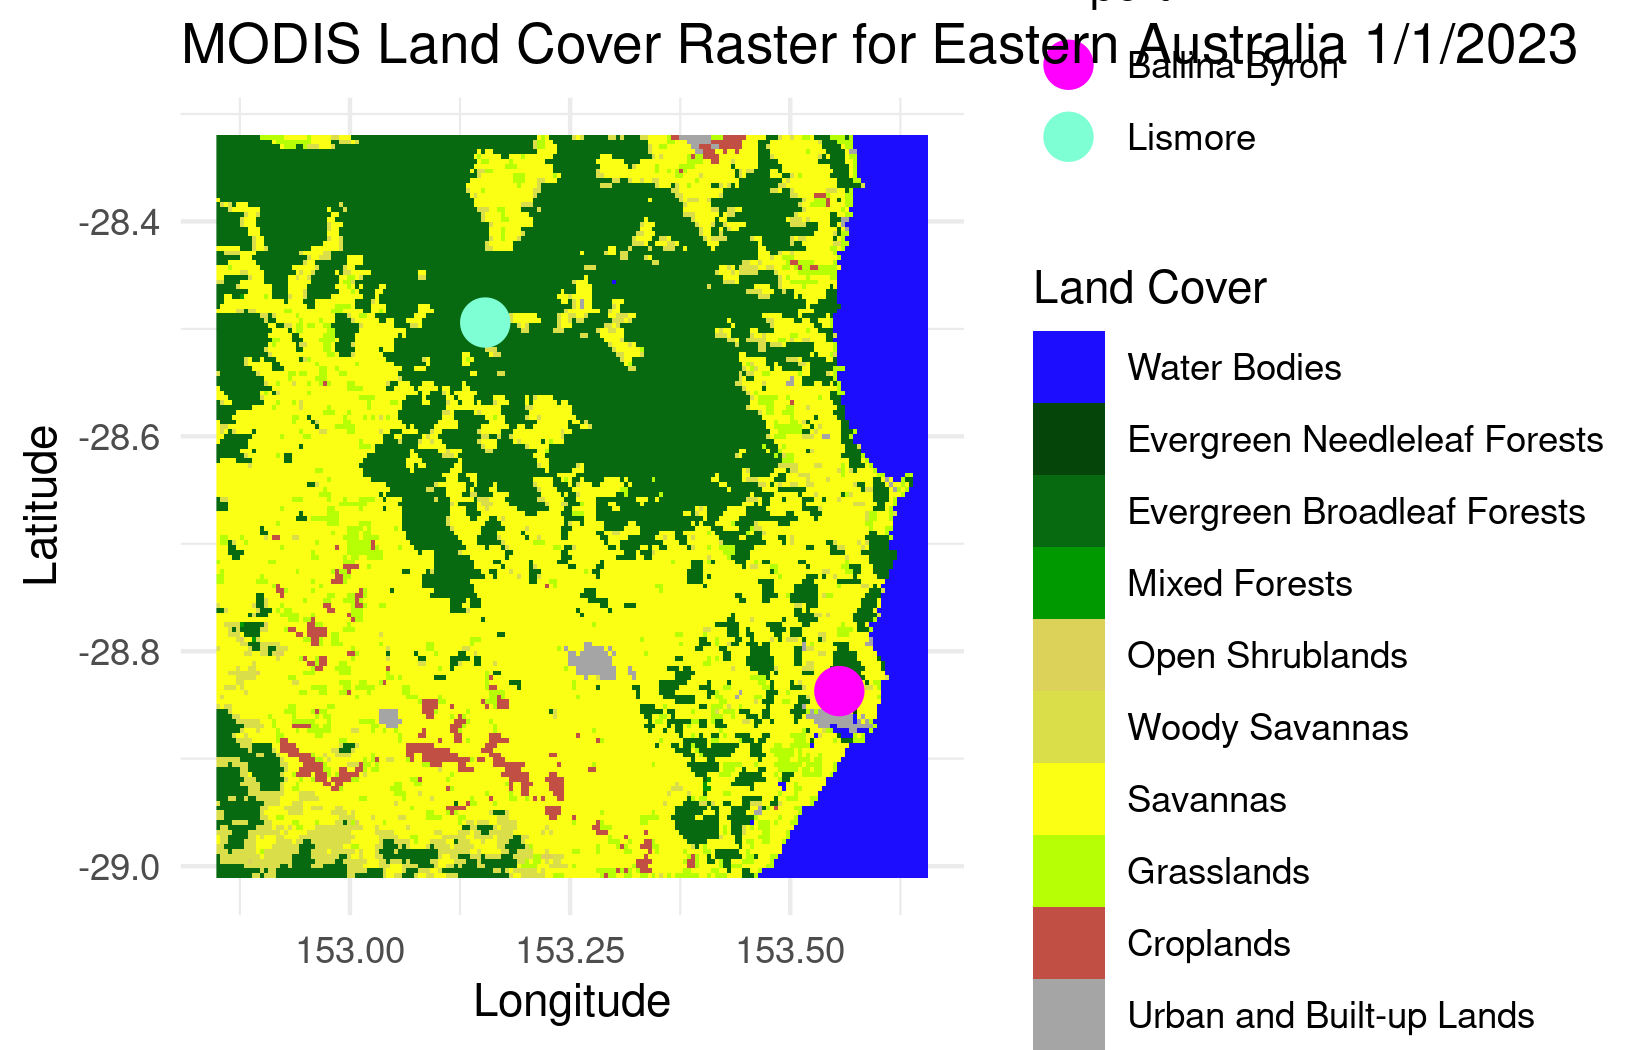
\includegraphics[keepaspectratio]{main_QMD_files/figure-pdf/unnamed-chunk-10-1.png}}

\section{Methods}\label{sec:methods}

\section{Conclusion}\label{sec:conclusion}

Amazing conclusions will be described in this section.


  \bibliography{references.bib}



\end{document}
